\section{Trasformazioni tra Sistemi di Riferimento}
Poiché le forze e quantità del velivolo saranno descritte in diversi sistemi di riferimento, è necessario convertirle in un unico sistema coerente per poterle utilizzare nelle equazioni del moto.
Di seguito sono descritte le matrici di trasformazione utilizzate nel corso di questa tesi.

\subsubsection{Trasformazione da Sistema NED a FRD}\label{subsec:Eulero}
La trasformazione tra due i sistemi di riferimento avviene attraverso tre rotazioni successive.
I tre angoli, detti angoli di Eulero, si definiscono come segue:
\begin{note}
    Sia $N$ un insieme di punti dato dall'intersezione tra i piani generati dalle coppie di vettori $\hat{x}_{NED}$ $\hat{y}_{NED}$ e $\hat{x}_{FRD}$ $\hat{y}_{FRD}$,
\end{note}
\begin{sitemize}
    \item $\psi$ è l'angolo di imbardata, ovvero l'angolo tra l'insieme di punti $N$ e l'asse $\hat{x}_{FRD}$.
    \item $\theta$ è l'angolo di beccheggio, ovvero l'angolo tra l'asse $\hat{z}_{NED}$ e l'asse $\hat{z}_{FRD}$.
    \item $\phi$ è l'angolo di rollio, ovvero l'angolo tra l'asse $\hat{x}_{NED}$ e l'insieme di punti $N$.
\end{sitemize}

\begin{figure}[H]
    \centering
    \includegraphics[width=0.35\linewidth]{Immagini/euler_angles.pdf}
    \caption{Trasformazione tra sistemi di riferimento con angoli di Eulero \cite{wiki:eulerangles}}
\end{figure}

La matrice di trasformazione tra i due sistemi di riferimento può essere definita effettuando 3 rotazioni seperate:
\begin{enumerate}
    \setlength{\itemsep}{0pt}
    \setlength{\parskip}{0pt}
    \setlength{\parsep}{0.25em}
    \setlength{\topsep}{0.5em}
    \setlength{\leftmargin}{1em}
    \setlength{\labelwidth}{1em}
    \setlength{\labelsep}{0.5em}
    \item Rotazione di $\psi$ attorno all'asse $\hat{z}_{FRD}$ descritta dalla matrice di rotazione $R_{z}(\psi)$

          Dato un generico punto $\begin{smallmatrix}(x_{NED}&y_{NED})\end{smallmatrix}$ è possibile scomporre le componenti in vettori lungo $\hat{x}_{FRD}$ e $\hat{y}_{FRD}$.
          \begin{figure}[H]
              \centering
              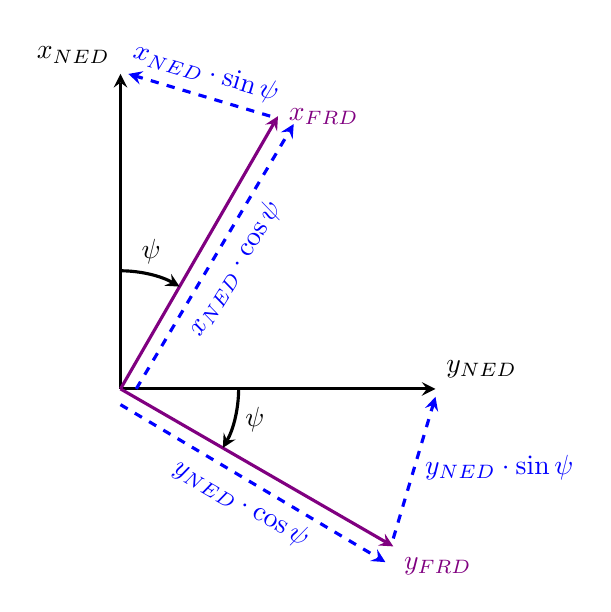
\begin{tikzpicture}[>=stealth, line width=0.4mm]

                  % Psi angle
                  \def\rotation{30}
                  \def\length{4}

                  % Coordinate axes
                  \coordinate (O) at (0,0);
                  \coordinate (xNED) at (0,\length);
                  \coordinate (yNED) at (\length,0);

                  % Rotated coordinates for FRD
                  \coordinate (xFRD) at ({\length*cos(\rotation)},{-\length*sin(\rotation)});
                  \coordinate (yFRD) at ({\length*sin(\rotation)},{\length*cos(\rotation)});

                  % NED frame
                  \draw[->, black] (O) -- (xNED) node[above left] {\textbf{$x_{NED}$}};
                  \draw[->, black] (O) -- (yNED) node[above right] {\textbf{$y_{NED}$}};

                  % FRD frame
                  \draw[->, violet] (O) -- (xFRD) node[below right] {\textbf{$y_{FRD}$}};
                  \draw[->, violet] (O) -- (yFRD) node[right] {\textbf{$x_{FRD}$}};

                  % Dashed projections for x_FRD
                  \draw[->, dashed, blue] ({\length*cos(\rotation)},{-\length*sin(\rotation) + 0.1}) -- (\length,-0.1) node[midway, right, blue] {$y_{NED} \cdot \sin \psi$};
                  \draw[->, dashed, blue] (0, -0.2) -- ({\length*cos(\rotation) - 0.1},{-\length*sin(\rotation) - 0.2}) node[midway, below, rotate=-\rotation, blue] {$y_{NED} \cdot \cos \psi$};

                  % Dashed projections for y_FRD
                  \draw[->, dashed, blue] ({\length*sin(\rotation) - 0.1},{\length*cos(\rotation)}) -- (0.1, \length) node[midway, above, rotate=-{\rotation/2-2}, blue] {$x_{NED} \cdot \sin \psi$};
                  \draw[->, dashed, blue] (0.2, 0) -- ({\length*sin(\rotation) + 0.2},{\length*cos(\rotation) - 0.1}) node[midway, below, rotate={\rotation*2 - 2}, blue] {$x_{NED} \cdot \cos \psi$};

                  % Angles
                  \draw[->] (1.5,0) arc[start angle=0,end angle=-\rotation,radius=1.5] node[midway, right] {$\psi$};

                  \draw[->] (0,1.5) arc[start angle=90,end angle=90-\rotation,radius=1.5]  node[midway, above] {$\psi$};

              \end{tikzpicture}
              \caption{Scomposizione delle componenti}
          \end{figure}


          Sommando poi le componenti proiettate sugli assi $\hat{x}_{FRD}$ e $\hat{y}_{FRD}$ si ottiene:
          \begin{equation*}
              R_{z}(\psi) = \begin{bmatrix}
                  \cos\psi & -\sin\psi & 0 \\
                  \sin\psi & \cos\psi  & 0 \\
                  0        & 0         & 1
              \end{bmatrix}
          \end{equation*}
    \item Rotazione di $\theta$ attorno all'asse $\hat{y}_{FRD}$ descritta dalla matrice di rotazione $R_{y}(\theta)$
          \begin{equation*}
              R_{y}(\theta) = \begin{bmatrix}
                  \cos\theta & 0 & -\sin\theta \\
                  0          & 1 & 0           \\
                  \sin\theta & 0 & \cos\theta
              \end{bmatrix}
          \end{equation*}
    \item Rotazione di $\phi$ attorno all'asse $\hat{x}_{FRD}$ descritta dalla matrice di rotazione $R_{x}(\phi)$
          \begin{equation*}
              R_{x}(\phi) = \begin{bmatrix}
                  1 & 0         & 0        \\
                  0 & \cos\phi  & \sin\phi \\
                  0 & -\sin\phi & \cos\phi \\
              \end{bmatrix}
          \end{equation*}
\end{enumerate}

La matrice di trasformazione completa è quindi data da:
\begin{multline}
    \label{eq:NEDtoFRD}
    C_{NED \rightarrow FRD} = R_{z}(\psi)R_{y}(\theta)R_{x}(\phi) = \\ = \begin{bmatrix}
        \cos\theta\cos\psi                            & \cos\theta\sin\psi                            & -\sin\theta        \\
        \sin\phi\sin\theta\cos\psi - \cos\phi\sin\psi & \sin\phi\sin\theta\sin\psi + \cos\phi\cos\psi & \sin\phi\cos\theta \\
        \cos\phi\sin\theta\cos\psi + \sin\phi\sin\psi & \cos\phi\sin\theta\sin\psi - \sin\phi\cos\psi & \cos\phi\cos\theta
    \end{bmatrix}
\end{multline}

\subsubsection{Trasformazione da Sistema FRD a NED}
Come riportato in \cite{smith_aircraft_flight_mechanics} la matrice di trasformazione $C_{NED \rightarrow FRD}$ è ortogonale, ovvero soddisfa la relazione $C_{NED \rightarrow FRD} \cdot C_{NED \rightarrow FRD}^T = I$.
Di conseguenza, la matrice inversa coincide con la trasposta:
\begin{multline}
    \label{eq:FRDtoNED}
    C_{FRD \rightarrow NED}  = C_{NED \rightarrow FRD}^T = \\
    = \begin{bmatrix}
        \cos\theta\cos\psi & \sin\phi\sin\theta\cos\psi + \cos\phi\sin\psi & \cos\phi\sin\theta\cos\psi - \sin\phi\sin\psi \\
        \cos\theta\sin\psi & \sin\phi\sin\theta\sin\psi - \cos\phi\cos\psi & \cos\phi\sin\theta\sin\psi + \sin\phi\cos\psi \\
        -\sin\theta        & \sin\phi\cos\theta                            & \cos\phi\cos\theta
    \end{bmatrix}
\end{multline}

\subsubsection{Trasformazione da Sistema Assi di Stabilità a FRD}
I due sistemi differiscono per una sola rotazione di un angolo $\alpha$ attorno all'asse $\hat{y}_{S}$. La matrice di trasformazione è definita similmente a quanto fatto per la rotazione di $\theta$ in \eqref{eq:NEDtoFRD}:
\begin{equation}
    \label{eq:StoFRD}
    C_{S \rightarrow FRD} = \begin{bmatrix}
        \cos\alpha & 0 & -\sin\alpha \\
        0          & 1 & 0           \\
        \sin\alpha & 0 & \cos\alpha
    \end{bmatrix}
\end{equation}

\subsubsection{Trasformazione da Sistema Assi Vento a FRD}
I due sistemi differiscono per due rotazioni: una di $\beta$ attorno all'asse $\hat{z}_{S}$ e una di $\alpha$ attorno all'asse $\hat{y}_{FRD}$. La matrice di rotazione è definita nel seguente modo, similmente a quanto fatto per la rotazione di $\psi$ in \eqref{eq:NEDtoFRD}:
\begin{equation}
    \label{eq:WtoFRD}
    \begin{split}
        C_{W \rightarrow FRD} & = \begin{bmatrix}
                                      \cos\alpha & 0 & -\sin\alpha \\
                                      0          & 1 & 0           \\
                                      \sin\alpha & 0 & \cos\alpha
                                  \end{bmatrix} \cdot \begin{bmatrix}
                                                          \cos\beta & -\sin\beta & 0 \\
                                                          \sin\beta & \cos\beta  & 0 \\
                                                          0         & 0          & 1
                                                      \end{bmatrix} \\ &= \begin{bmatrix}
            \cos\alpha\cos\beta & -\cos\alpha\sin\beta & -\sin\alpha \\
            \sin\beta           & \cos\beta            & 0           \\
            \sin\alpha\cos\beta & -\sin\alpha\sin\beta & \cos\alpha
        \end{bmatrix}
    \end{split}
\end{equation}
